\documentclass{beamer}

% \usetheme{AnnArbor}
\usetheme{Singapore}
\usecolortheme{dolphin}

\mode<presentation>

\usepackage{xspace}
\usepackage{multicol}
\usepackage{amssymb}
\usepackage{tabularx}
\usepackage{wasysym}
\usepackage{graphicx}
\usepackage{multirow}
\usepackage{mathtools}
\usepackage[style=authoryear,backend=biber]{biblatex}
\usepackage{wrapfig}
\usepackage{listings}

\usepackage{keystroke}  %% \Return
% \usepackage{menukeys} 
% \verb|\Return| \Return % from package keystroke

\newcommand{\vs}{\vspace{0.5cm}}

\graphicspath{{./graphs/}{./imgs/}{./photos/}
}
\DeclareGraphicsExtensions{.eps}

% \AtBeginSection{\frame{\sectionpage}}
\AtBeginSection[] % Do nothing for \section*
{
\begin{frame}<beamer>
\frametitle{Outline}
\tableofcontents[currentsection]
\end{frame}
}
\setbeamertemplate{footline}[frame number]

\include{colour}
\include{layout-text}
\include{layout-tables}

\begin{document}


\title{Snakemake}
\author{Raymond Wan}
\date{July 14, 2018}

\maketitle


%%%%%%%%%%%%%%%%%%%%%%%%%%%%%%%%%%%%%%%%%%%%%%%%%%%%%%%
\section{Introduction}


%%%%%%%%%%%%%%%%%%%%%%%%%%%%%%%%%%%%%%%%%%%%%%%%%%%%%%%
%%%%%%%%%%%%%%%%%%%%%%%%%%%%%%%%%%%%%%%%%%%%%%%%%%%%%%%
\begin{frame}

\frametitle{Overview}

Snakemake is:
\begin{itemize}
  \item A {\red{workflow}} definition language, similar to Make.
  \item Based on {\green{Python}}.
  \item Developed for bioinformatics\footnote{The application of computer science, statistics, etc. to problems in the life sciences.}, but general enough for other tasks.
\end{itemize}

\end{frame}


%%%%%%%%%%%%%%%%%%%%%%%%%%%%%%%%%%%%%%%%%%%%%%%%%%%%%%%
\begin{frame}

\frametitle{Disclaimer}

\begin{quotation}
In terms of scripts, I'm primarily a Perl programmer and have had to learn Python the past year because of Snakemake.  Thus, I don't claim to be an expert of either Python or Snakemake.  I will cover what I've needed to know (so far).
\vs

Hopefully this talk will give you enough information to decide if Snakemake is useful for your work.
\end{quotation}

\end{frame}


%%%%%%%%%%%%%%%%%%%%%%%%%%%%%%%%%%%%%%%%%%%%%%%%%%%%%%%
\begin{frame}

\frametitle{Pipelines}

Like other areas of data analysis, bioinformaticians often chain a series of programs together so that the output of one program becomes the input of another:

\begin{figure}
  \centering
  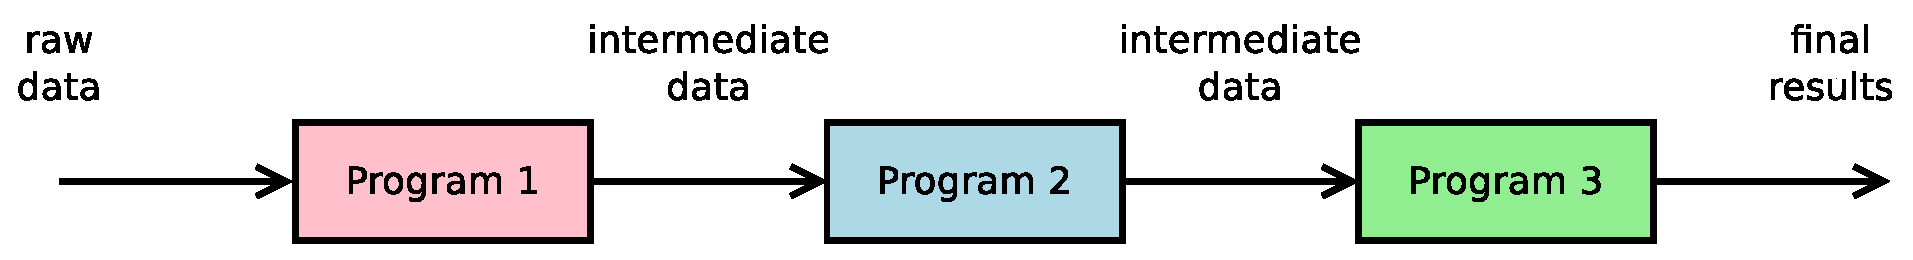
\includegraphics[width=\linewidth]{intro/pipeline-ex}
\end{figure}

\end{frame}


%%%%%%%%%%%%%%%%%%%%%%%%%%%%%%%%%%%%%%%%%%%%%%%%%%%%%%%
\begin{frame}[fragile]

\frametitle{Make}

For longer than what some of us are willing to admit \smiley, we may have used Make to build programs and libraries from source code.\\
\vs

Files with the filename {\texttt{Makefile}} are used with rules of this form:

\begin{figure}
  \centering
\begin{lstlisting}[language=make]
target:  dependencies
    system command(s)
\end{lstlisting}
\end{figure}

\end{frame}


%%%%%%%%%%%%%%%%%%%%%%%%%%%%%%%%%%%%%%%%%%%%%%%%%%%%%%%
\begin{frame}[fragile]

\frametitle{Make}

Thus, a rule in a Makefile might look like this:

\begin{figure}
  \centering
\begin{lstlisting}[language=make]
helloworld:  helloworld.c
	gcc helloworld.c -o helloworld
\end{lstlisting}
\end{figure}

When compiling a program with a Makefile, you might be using one compiler to compile source files to object files, linking them, and maybe even doing this in parallel.

\end{frame}


%%%%%%%%%%%%%%%%%%%%%%%%%%%%%%%%%%%%%%%%%%%%%%%%%%%%%%%
\begin{frame}

\frametitle{Galaxy}

Not surprisingly, bioinformaticians have developed their own systems (too numerous to list them all) which ultimately do almost the same thing (from a computing perspective).
\vs

Galaxy (which predates Snakemake) is a web-based system for constructing such workflows.

\end{frame}


%%%%%%%%%%%%%%%%%%%%%%%%%%%%%%%%%%%%%%%%%%%%%%%%%%%%%%%
\begin{frame}

\frametitle{Galaxy}

\begin{figure}
  \centering
  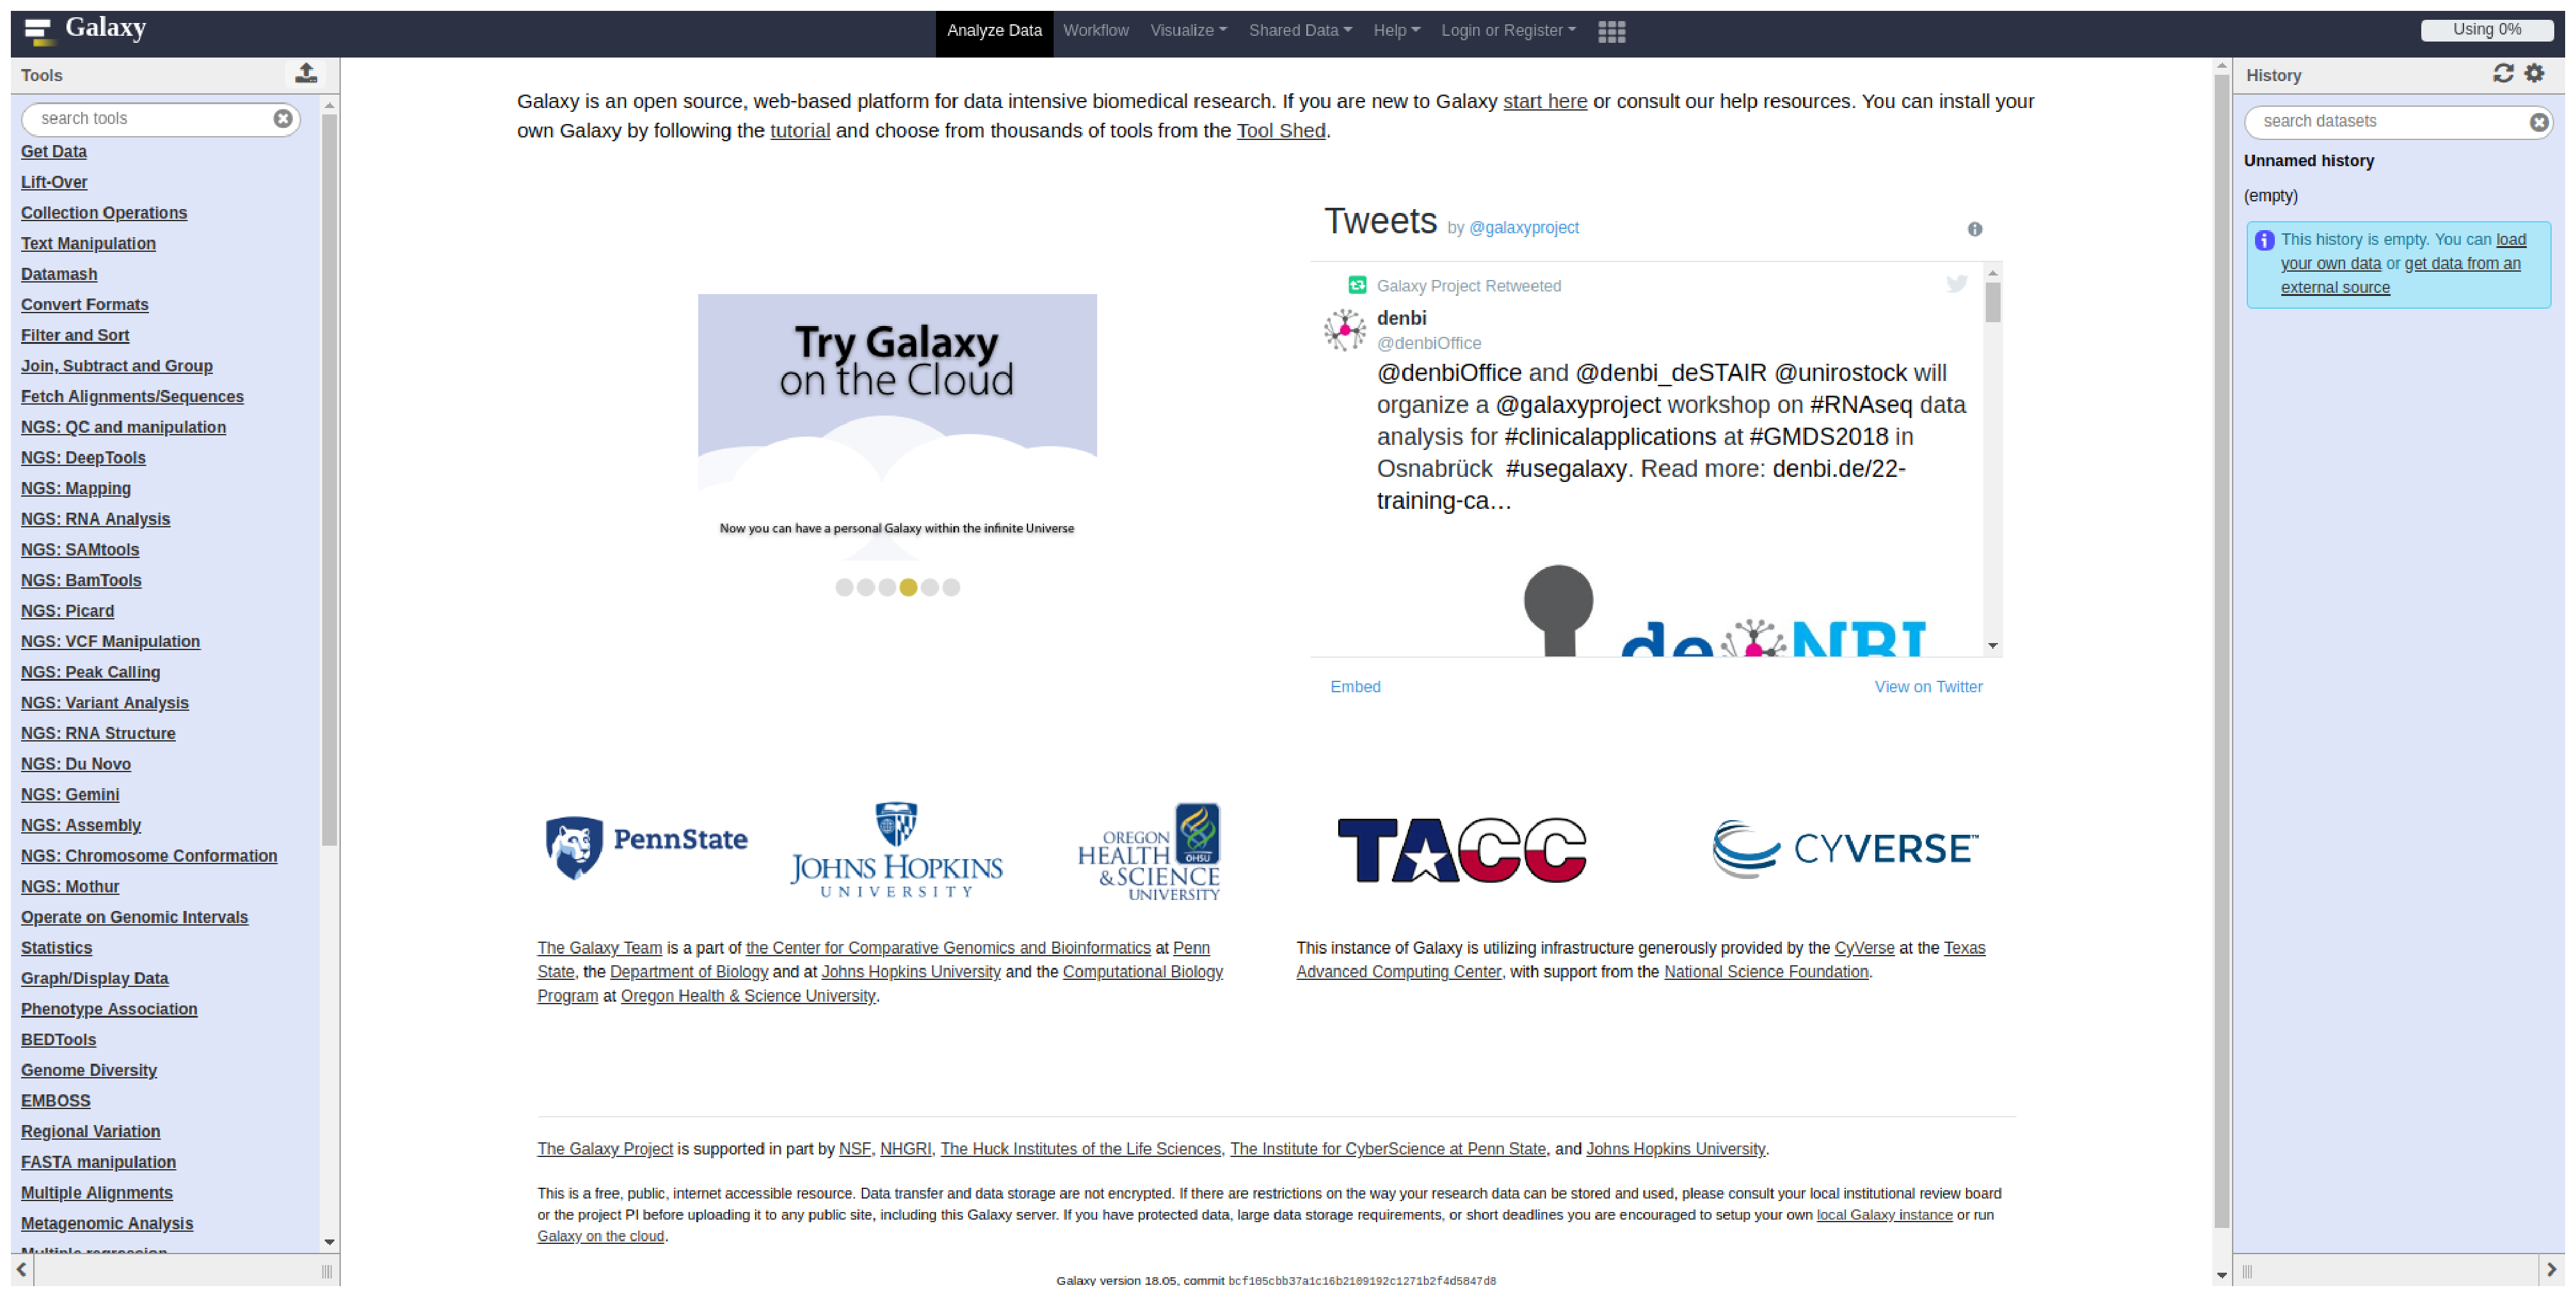
\includegraphics[width=\linewidth]{intro/galaxy-0}
\end{figure}

{\figsource{\href{https://usegalaxy.org/}{https://usegalaxy.org/}}}

\end{frame}


%%%%%%%%%%%%%%%%%%%%%%%%%%%%%%%%%%%%%%%%%%%%%%%%%%%%%%%
\begin{frame}

\frametitle{Galaxy}

\begin{figure}
  \centering
  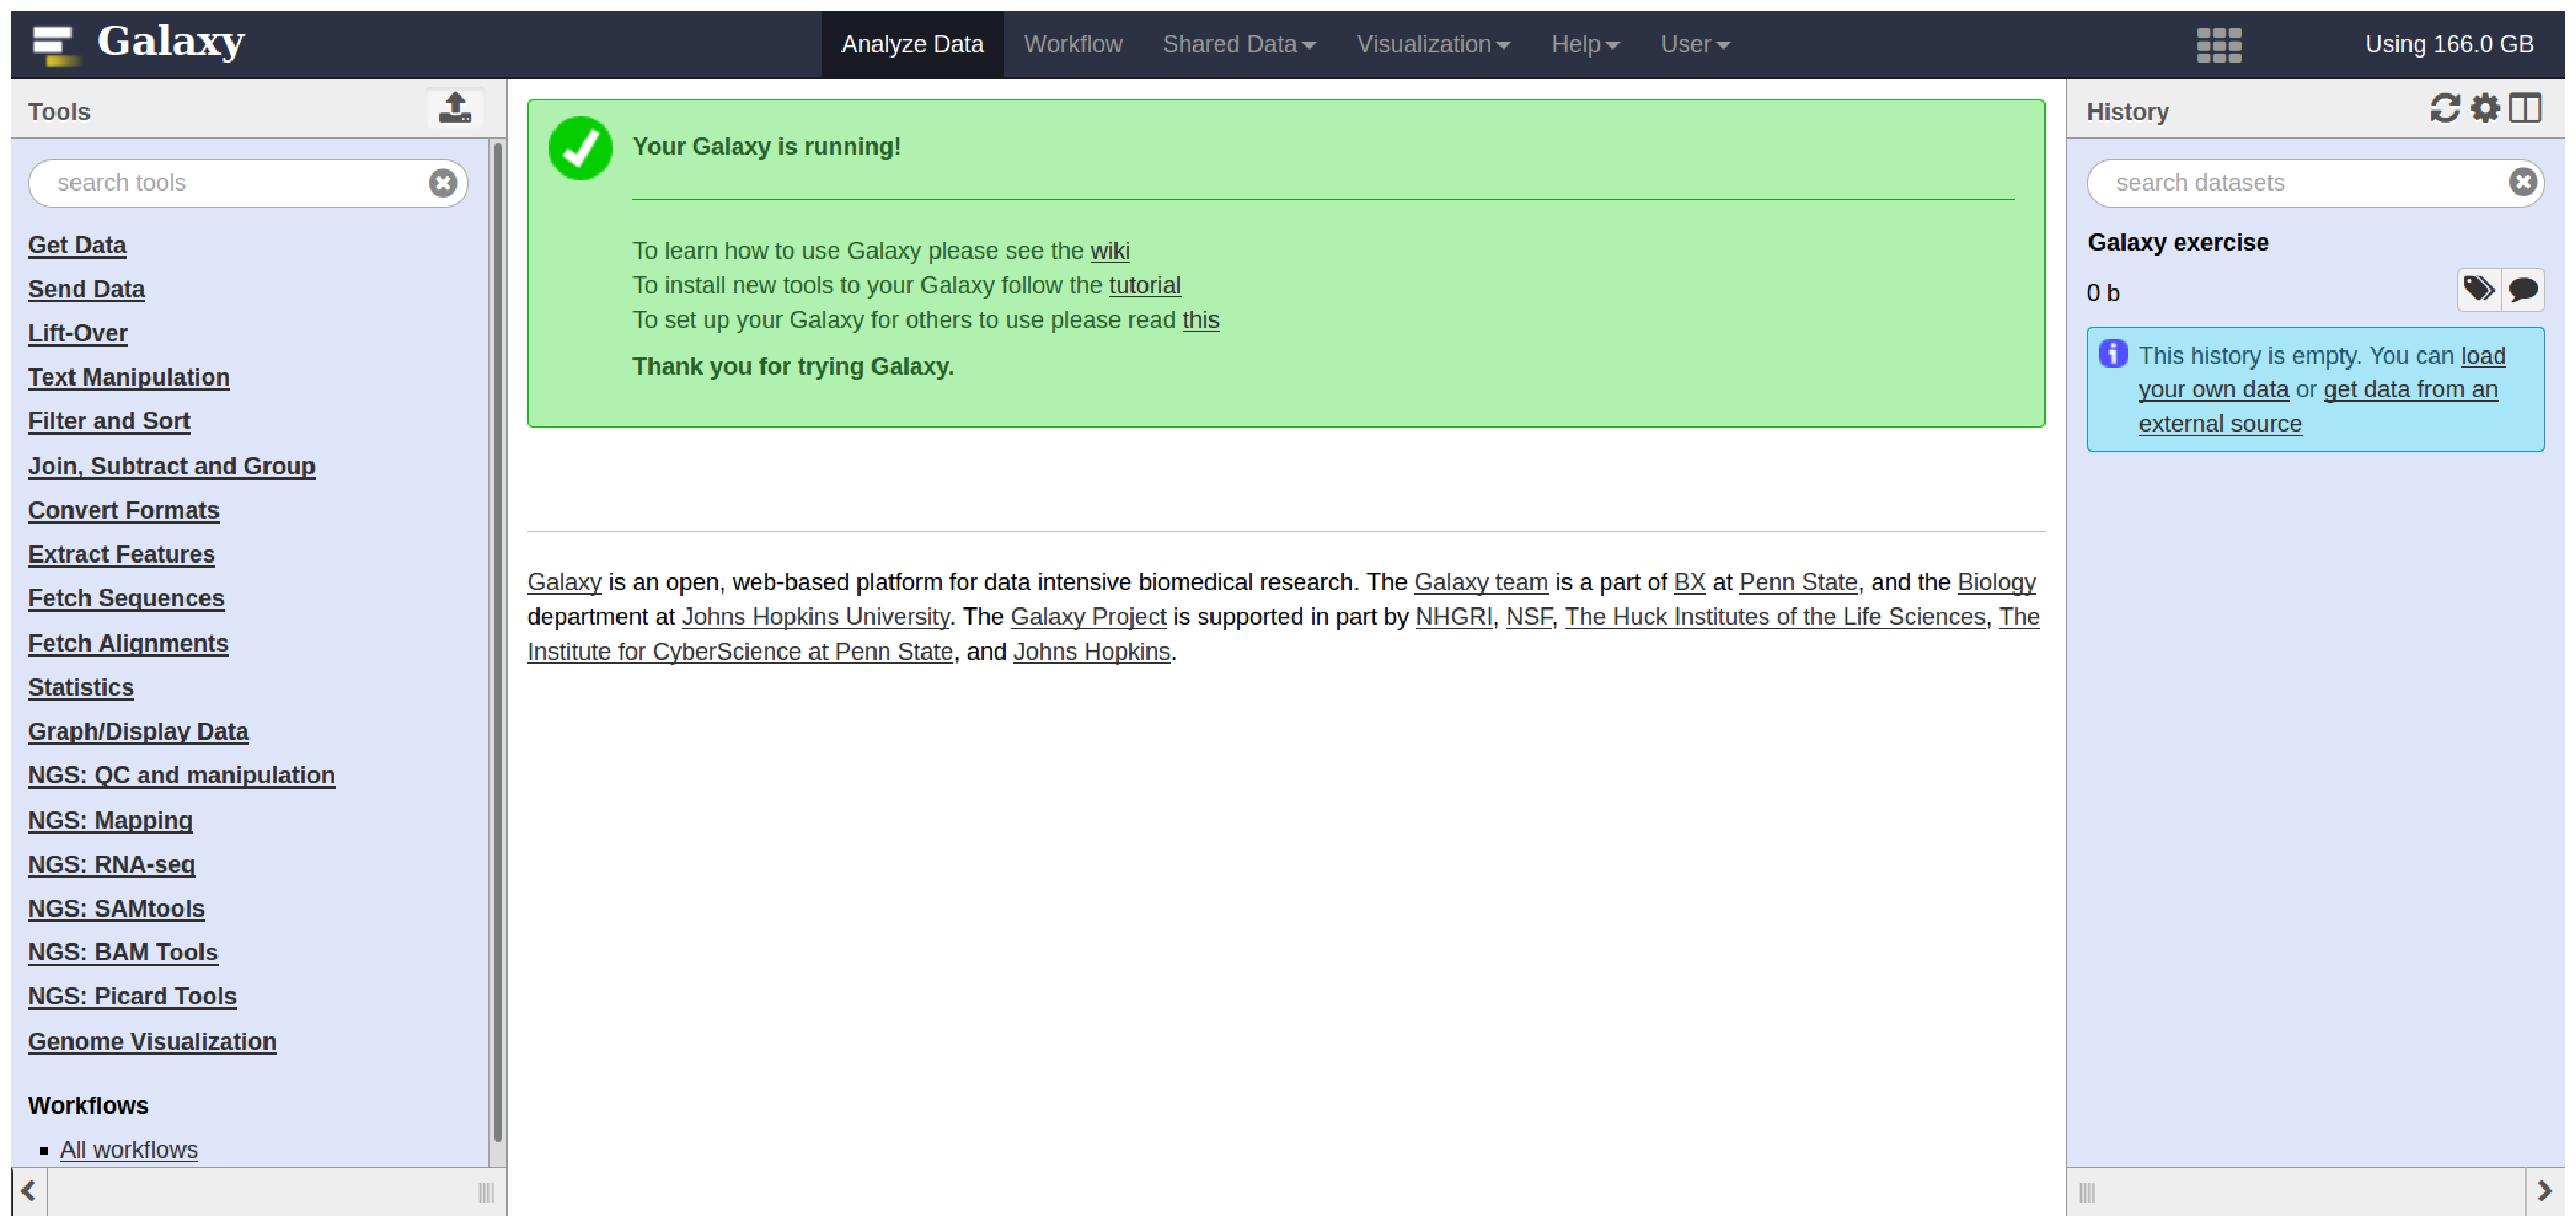
\includegraphics[width=\linewidth]{intro/galaxy-1}
\end{figure}

{\figsource{Local installation}}

\end{frame}


%%%%%%%%%%%%%%%%%%%%%%%%%%%%%%%%%%%%%%%%%%%%%%%%%%%%%%%
\begin{frame}

\frametitle{Galaxy}

\begin{figure}
  \centering
  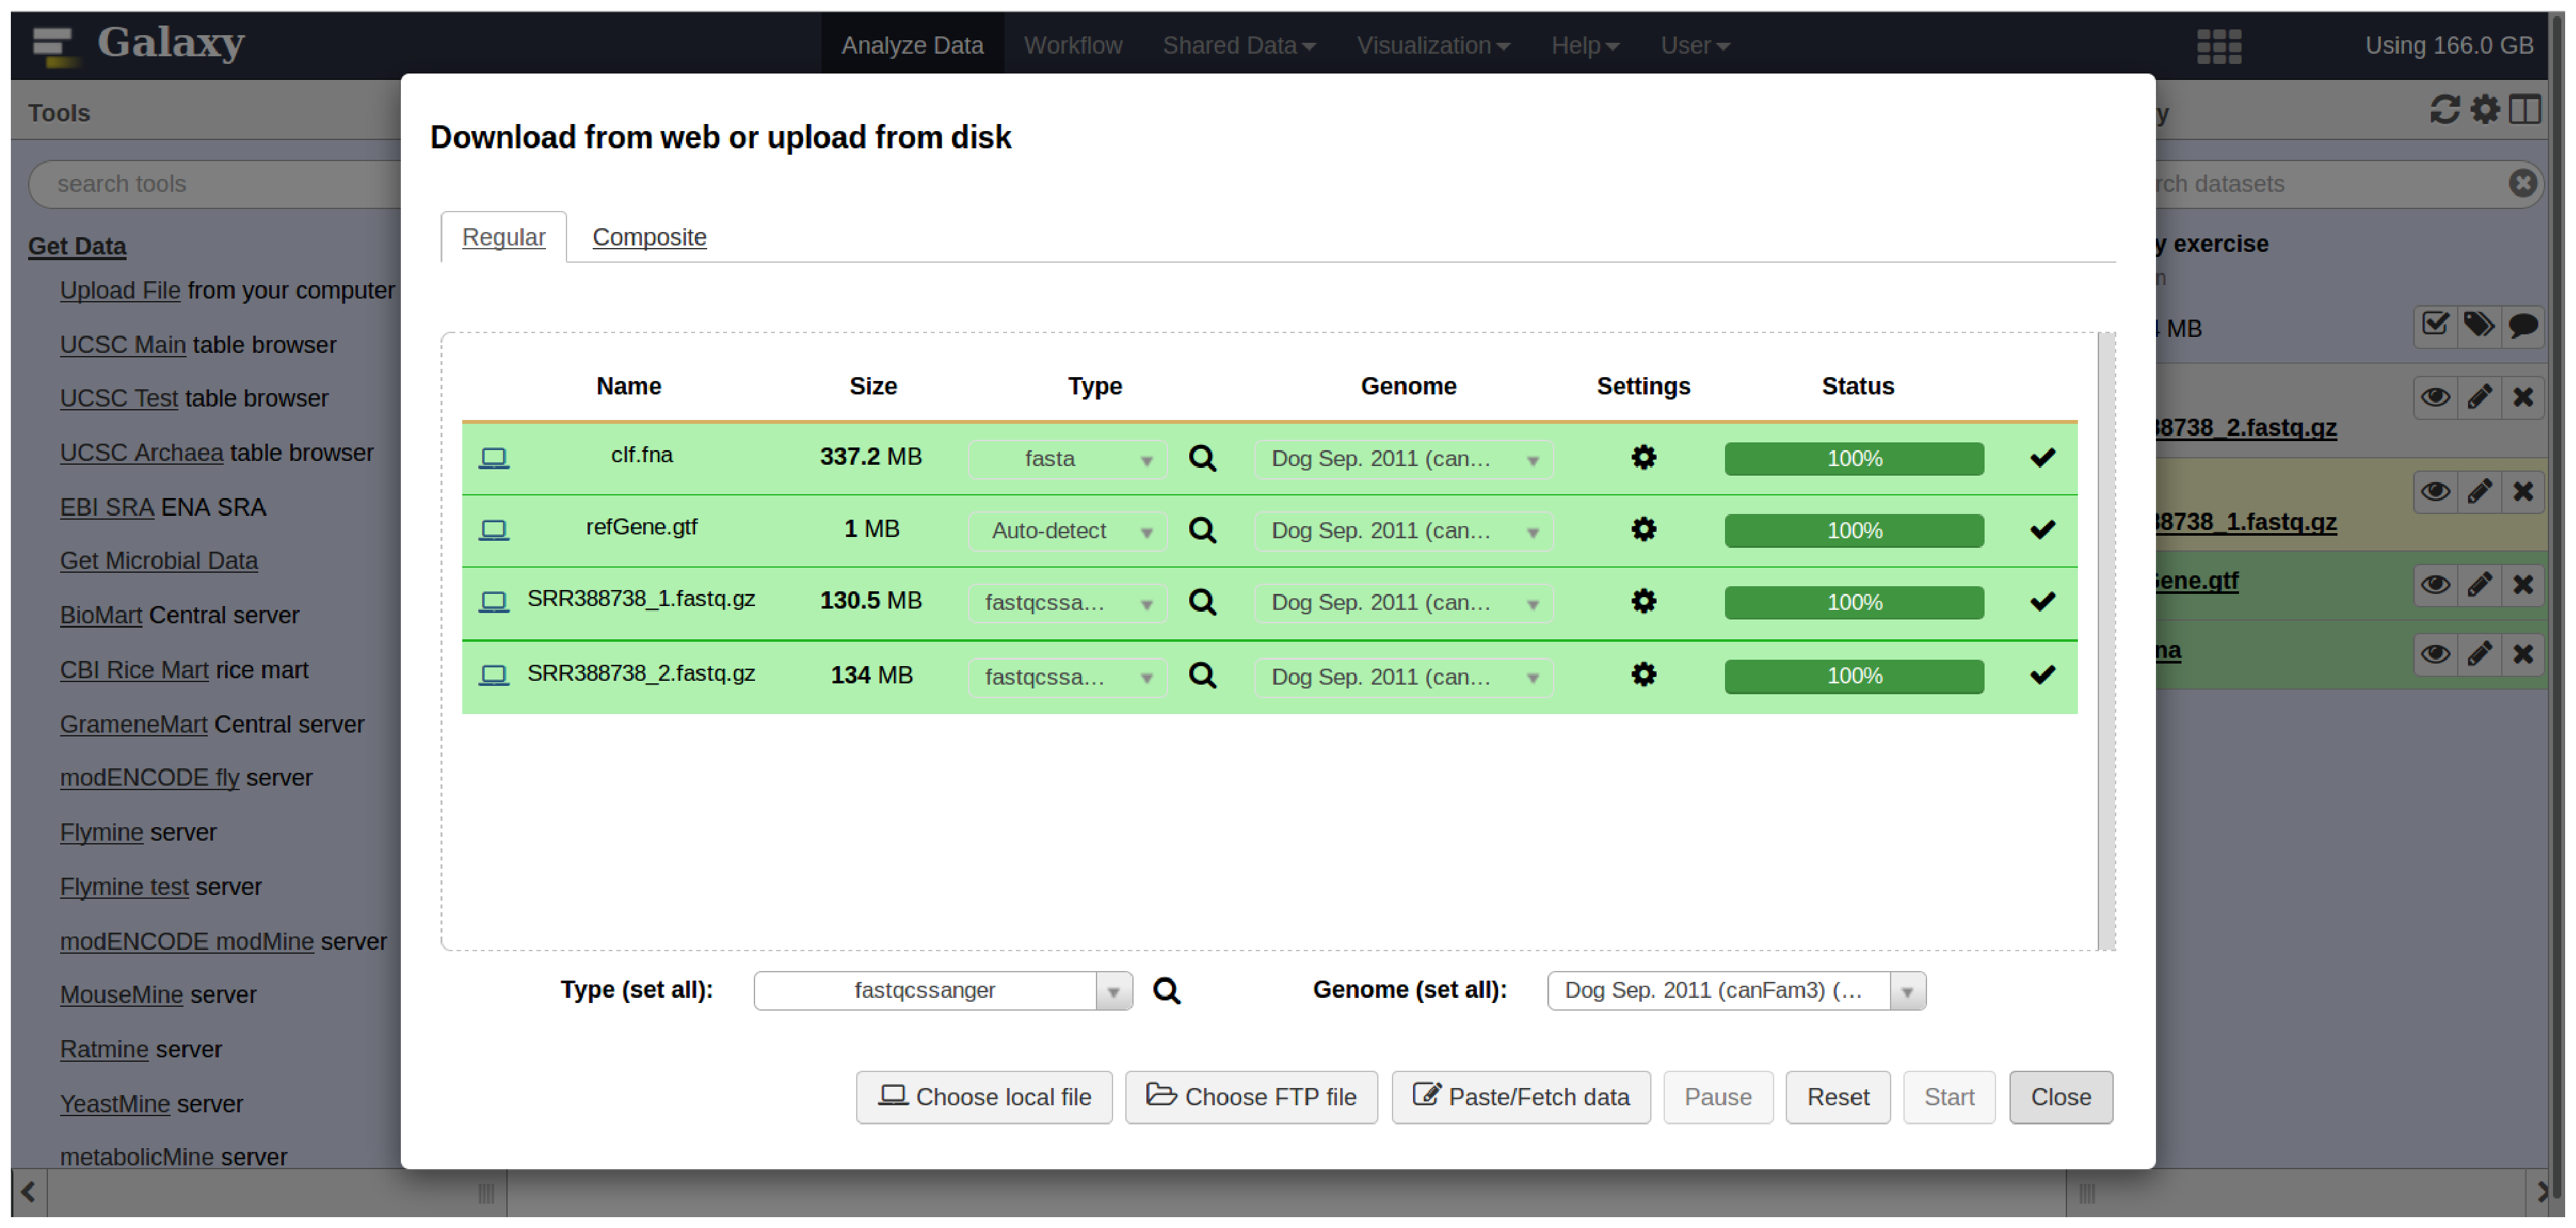
\includegraphics[width=\linewidth]{intro/galaxy-2}
\end{figure}

\end{frame}


%%%%%%%%%%%%%%%%%%%%%%%%%%%%%%%%%%%%%%%%%%%%%%%%%%%%%%%
\begin{frame}

\frametitle{Galaxy}

\begin{figure}
  \centering
  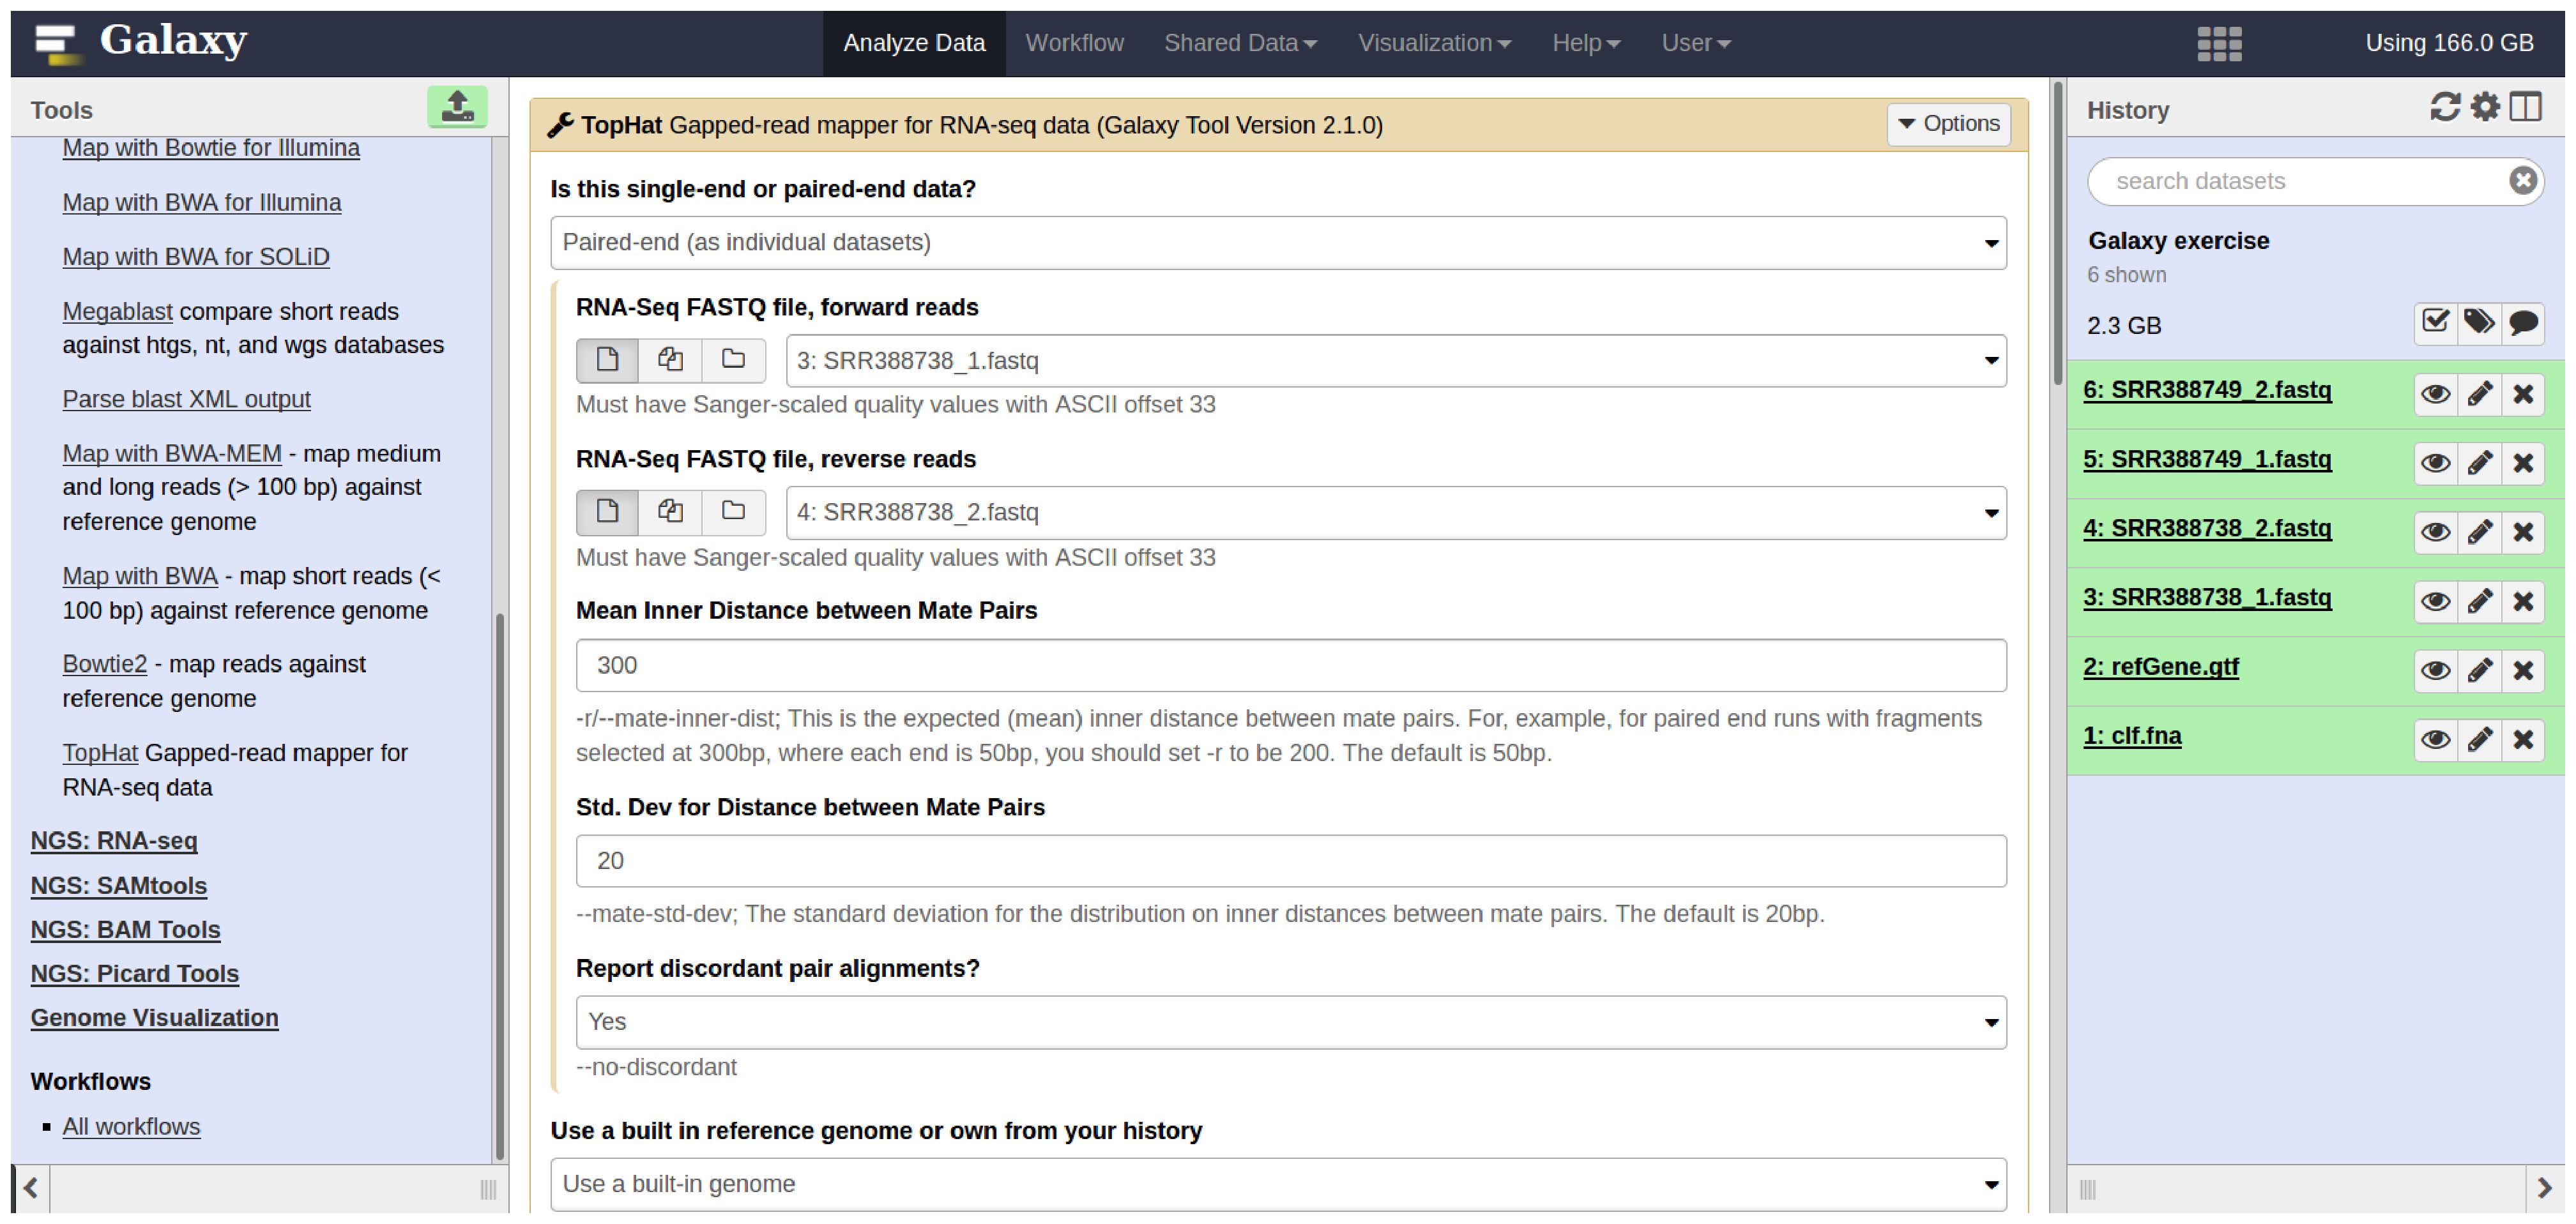
\includegraphics[width=\linewidth]{intro/galaxy-3}
\end{figure}

\end{frame}


%%%%%%%%%%%%%%%%%%%%%%%%%%%%%%%%%%%%%%%%%%%%%%%%%%%%%%%
\begin{frame}

\frametitle{Galaxy}

\begin{figure}
  \centering
  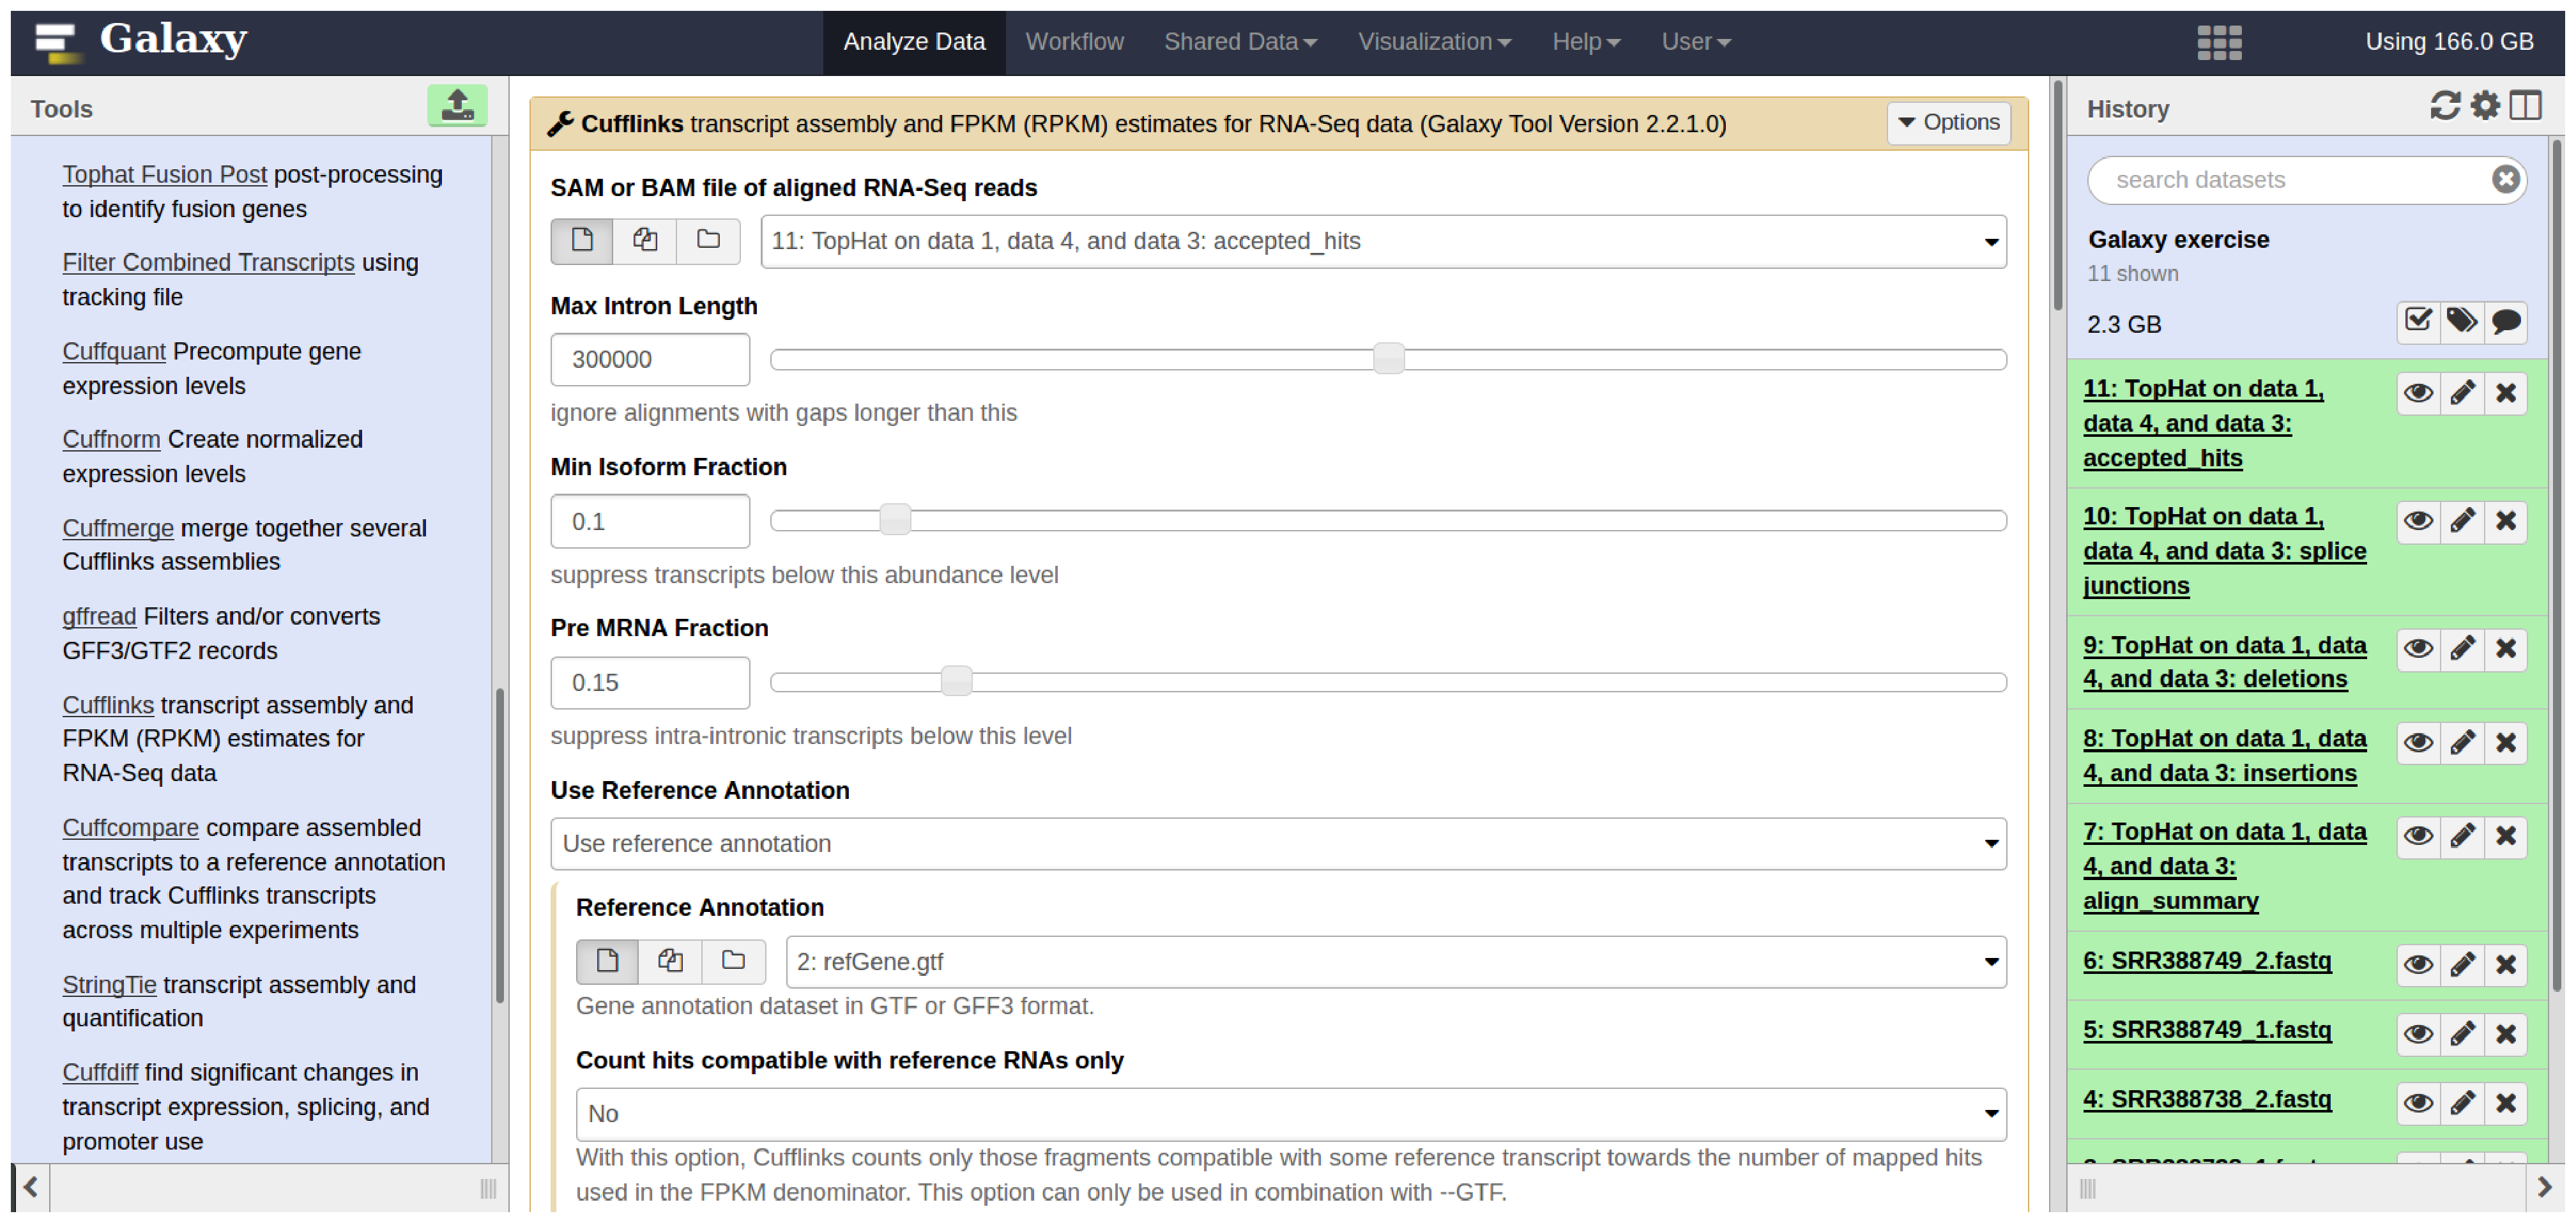
\includegraphics[width=\linewidth]{intro/galaxy-4}
\end{figure}

While it's conceivable to generalize Galaxy for non-bioinformaticians, it's probably not worth the effort...

\end{frame}


%%%%%%%%%%%%%%%%%%%%%%%%%%%%%%%%%%%%%%%%%%%%%%%%%%%%%%%
\begin{frame}

\frametitle{Snakemake}

Published in 2012 in the context of bioinformatics:

\begin{figure}
  \centering
  
\includegraphics[width=\linewidth]{imgs/kr12-bio-cover}
\end{figure}

This (unfortunately) undersells it since users who want to do what Make does, would appreciate its Python-based syntax.

\end{frame}





%%%%%%%%%%%%%%%%%%%%%%%%%%%%%%%%%%%%%%%%%%%%%%%%%%%%%%%
\section{Basics}


%%%%%%%%%%%%%%%%%%%%%%%%%%%%%%%%%%%%%%%%%%%%%%%%%%%%%%%
%%%%%%%%%%%%%%%%%%%%%%%%%%%%%%%%%%%%%%%%%%%%%%%%%%%%%%%
\begin{frame}

\frametitle{Rules}

A Snakemake workflow consists of a Snakemake file ({\texttt{Snakefile}}) that consists of a set of rules.
\vs

Each rule specifies a series of {\blue{directives}}, which includes at least:
\begin{enumerate}
  \item input files,
  \item output files, and
  \item how to generate the output files from the input files
\end{enumerate}
\vs

In many ways, this is similar to Make and Galaxy.

\end{frame}


%%%%%%%%%%%%%%%%%%%%%%%%%%%%%%%%%%%%%%%%%%%%%%%%%%%%%%%
\begin{frame}[fragile]

\frametitle{Sample Rule}

Save the following in {\texttt{Snakefile}}:
\begin{figure}
  \centering
  \begin{tabular}{lc}
%   rule HelloWorld: & \action<+->{{\red{$\leftarrow$}}} \\
  rule HelloWorld: & \only<1>{{\red{$\leftarrow$}}} \\
  {\D\D}input:  "Download/iris.data" & \only<2>{{\red{$\leftarrow$}}} \\
  {\D\D}output:  "HelloWorld/iris.txt" & \only<3>{{\red{$\leftarrow$}}} \\
  {\D\D}shell: & \only<4>{{\red{$\leftarrow$}}} \\
  {\D\D\D\D}""" & \only<5>{{\red{$\leftarrow$}}} \\
  {\D\D\D\D}./helloworld \{input\} {\textgreater}\{output\} & \only<6>{{\red{$\leftarrow$}}} \\
  {\D\D\D\D}"""  & \only<5>{{\red{$\leftarrow$}}} \\
  \end{tabular}
\end{figure}

Note:  Variables are enclosed in curly braces.

\end{frame}



%%%%%%%%%%%%%%%%%%%%%%%%%%%%%%%%%%%%%%%%%%%%%%%%%%%%%%%
\begin{frame}[fragile]

\frametitle{Sample Rule}

{\magenta{\$  }}  {\texttt{snakemake HelloWorld/iris.txt}}
{\tiny{
\begin{figure}
  \centering
  \begin{tabular}{l}
Building DAG of jobs... \\
Provided cores: 1 \\
Rules claiming more threads will be scaled down. \\
Job counts: \\
	count	jobs \\
	1	HelloWorld \\
	1 \\
 \\
rule HelloWorld: \\
    input: Download/iris.data \\
    output: HelloWorld/iris.txt \\
    jobid: 0 \\
 \\
Finished job 0. \\
1 of 1 steps (100\%) done \\
  \end{tabular}
\end{figure}
}}

\end{frame}


%%%%%%%%%%%%%%%%%%%%%%%%%%%%%%%%%%%%%%%%%%%%%%%%%%%%%%%
\begin{frame}[fragile]

\frametitle{Sample Rule}

If the input doesn't exist, then the command will not work:
\vs

{\magenta{\$  }}  {\texttt{snakemake HelloWorld/not-exist.txt}}
\begin{figure}
  \centering
  \begin{tabular}{l}
Building DAG of jobs... \\
MissingInputException in line 1 of Snakefile.py: \\
Missing input files for rule HelloWorld: \\
Download/not-exist.data \\
  \end{tabular}
\end{figure}

Not surprisingly, the {\blue{input}} directive is a precondition for the rule to run.

\end{frame}


%%%%%%%%%%%%%%%%%%%%%%%%%%%%%%%%%%%%%%%%%%%%%%%%%%%%%%%
\begin{frame}

\frametitle{Variable Substitution}

The interesting part of Snakemake (IMHO) occurs during variable substitution; commands can then be generalized.

\end{frame}


%%%%%%%%%%%%%%%%%%%%%%%%%%%%%%%%%%%%%%%%%%%%%%%%%%%%%%%
\begin{frame}

\frametitle{Variable Substitution}

\begin{figure}
  \centering
  \begin{tabular}{lc}
  rule HelloWorld: & \\
  {\D\D}input:  "Download/\{dataset\}.data" & \only<2>{{\red{$\leftarrow$}}} \\
  {\D\D}output:  "HelloWorld/\{dataset\}.txt" & \only<1>{{\red{$\leftarrow$}}} \\
  {\D\D}shell: & \\
  {\D\D\D\D}""" & \\
  {\D\D\D\D}./helloworld \{input\} {\textgreater}\{output\} & \\
  {\D\D\D\D}"""  & \\
  \end{tabular}
\end{figure}


\end{frame}


%%%%%%%%%%%%%%%%%%%%%%%%%%%%%%%%%%%%%%%%%%%%%%%%%%%%%%%
\begin{frame}[fragile]

\frametitle{Variable Substitution}

For example:
\vs

\begin{itemize}
  \item {\magenta{\$  }}  {\texttt{snakemake HelloWorld/abalone.txt}}
  \item {\magenta{\$  }}  {\texttt{snakemake HelloWorld/iris.txt}}
\end{itemize}
\vs

will both work as expected.

\end{frame}


%%%%%%%%%%%%%%%%%%%%%%%%%%%%%%%%%%%%%%%%%%%%%%%%%%%%%%%
\begin{frame}

\frametitle{Top-level Rule}

Instead of typing {\texttt{snakemake}} followed by the output to be generated every time, like Make, there is a top-level rule called {\texttt{all}}.
\vs

It is special in that it has {\red{no}} output defined.

\end{frame}


%%%%%%%%%%%%%%%%%%%%%%%%%%%%%%%%%%%%%%%%%%%%%%%%%%%%%%%
\begin{frame}

\frametitle{Top-level Rule}

\begin{figure}
  \centering
  \begin{tabular}{lc}
  rule all: \\
  {\D\D}input:  "HelloWorld/iris.txt" & \only<3>{{\red{$\leftarrow$}}} \\
  \\
  rule HelloWorld: & \\
  {\D\D}input:  "Download/\{dataset\}.data" & \only<2>{{\red{$\leftarrow$}}} \\
  {\D\D}output:  "HelloWorld/\{dataset\}.txt" & \only<1>{{\red{$\leftarrow$}}} \\
  {\D\D}shell: & \\
  {\D\D\D\D}""" & \\
  {\D\D\D\D}./helloworld \{input\} {\textgreater}\{output\} & \\
  {\D\D\D\D}"""  & \\
  \end{tabular}
\end{figure}

Note:  The {\texttt{all}} rule must come first.

\end{frame}


%%%%%%%%%%%%%%%%%%%%%%%%%%%%%%%%%%%%%%%%%%%%%%%%%%%%%%%
\begin{frame}

\frametitle{Top-level Rule}

{\magenta{\$  }}  {\texttt{snakemake}}
{\tiny{
\begin{figure}
  \centering
  \begin{tabular}{l}
Building DAG of jobs... \\
Provided cores: 1 \\
Rules claiming more threads will be scaled down. \\
Job counts: \\
	count	jobs \\
	1	HelloWorld \\
	1	all \\
	2 \\
 \\
rule HelloWorld: \\
    input: Download/iris.data \\
    output: HelloWorld/iris.txt \\
    jobid: 1 \\
    wildcards: dataset=iris \\
 \\
Finished job 1. \\
1 of 2 steps (50\%) done \\
 \\
localrule all: \\
    input: HelloWorld/iris.txt \\
    jobid: 0 \\
 \\
Finished job 0. \\
2 of 2 steps (100\%) done \\
  \end{tabular}
\end{figure}
}}

\end{frame}


%%%%%%%%%%%%%%%%%%%%%%%%%%%%%%%%%%%%%%%%%%%%%%%%%%%%%%%
\begin{frame}

\frametitle{Multiple Arguments}

\begin{figure}
  \centering
  \begin{tabular}{lc}
  rule HelloWorld: & \\
  {\D\D}input:  "Download/iris.data", \\
  {\D\D\D\D\D\D\D\D}"Download/abalone.data" \\
  {\D\D}output:  "HelloWorld/iris.txt" \\
  {\D\D}shell: \\
  {\D\D\D\D}""" \\
  {\D\D\D\D}\#\#  Assuming helloworld takes two arguments \\
  {\D\D\D\D}./helloworld \{input\} {\textgreater}\{output\} & \only<1>{{\red{$\leftarrow$}}} \\
  {\D\D\D\D}./helloworld \{input[0]\} \{input[1]\} {\textgreater}\{output\} & \only<2>{{\red{$\leftarrow$}}} \\
  {\D\D\D\D}""" \\
  \end{tabular}
\end{figure}

\end{frame}


%%%%%%%%%%%%%%%%%%%%%%%%%%%%%%%%%%%%%%%%%%%%%%%%%%%%%%%
\begin{frame}

\frametitle{Named Inputs/Outputs}

\begin{figure}
  \centering
  \begin{tabular}{lc}
  rule HelloWorld: & \\
  {\D\D}input: \\
  {\D\D\D\D}data1 = "Download/iris.data", \\
  {\D\D\D\D}data2 = "Download/abalone.data" \\
  {\D\D}output:  "HelloWorld/iris.txt" \\
  {\D\D}shell: \\
  {\D\D\D\D}""" \\
  {\D\D\D\D}./helloworld \{input.data2\} {\textgreater}\{output\} & \only<1>{{\red{$\leftarrow$}}} \\
  {\D\D\D\D}""" \\
  \end{tabular}
\end{figure}

\end{frame}


%%%%%%%%%%%%%%%%%%%%%%%%%%%%%%%%%%%%%%%%%%%%%%%%%%%%%%%
\begin{frame}

\frametitle{Parameters}

Within a rule, you might need access to non-file parameters for some reason.  This is where the {\blue{params}} directive is needed:
% {\small{
\begin{figure}
  \centering
  \begin{tabular}{lc}
  rule HelloWorld: \\
  {\D\D}input:  "Download/\{dataset\}.data" \\
  {\D\D}output:  "HelloWorld/\{dataset\}.txt" \\
  {\D\D}params: & \only<1>{{\red{$\leftarrow$}}} \\
  {\D\D}{\D\D}count="42", & \only<2>{{\red{$\leftarrow$}}} \\
  {\D\D}{\D\D}dataset="\{dataset\}" & \only<2>{{\red{$\leftarrow$}}} \\
  {\D\D}shell: \\
  {\D\D}{\D\D}""" \\
  {\D\D}{\D\D}./helloworld --count \{params.count\} --label {\Return} & \only<3>{{\red{$\leftarrow$}}} \\
  {\D\D}{\D\D}{\D\D}\{params.dataset\} \{input\} {\textgreater}\{output\} & \only<3>{{\red{$\leftarrow$}}} \\
  {\D\D}{\D\D}""" \\
  \end{tabular}
\end{figure}

\end{frame}


%%%%%%%%%%%%%%%%%%%%%%%%%%%%%%%%%%%%%%%%%%%%%%%%%%%%%%%
\begin{frame}

\frametitle{Functions for Inputs}

Instead of listing the inputs within a rule, a Python function that returns a list can be used.  ({\red{Finally}}, some Python...  \smiley)
\vs

Functions cannot be defined for outputs, though.

\end{frame}


%%%%%%%%%%%%%%%%%%%%%%%%%%%%%%%%%%%%%%%%%%%%%%%%%%%%%%%
\begin{frame}

\frametitle{Functions for Inputs}

{\small{
\begin{figure}
  \centering
  \begin{tabular}{lc}
  OUTPUT\_DIR = "Download/" & \only<7>{{\red{$\leftarrow$}}} \\
  \\
  def Get\_Inputs (foo): & \only<4>{{\red{$\leftarrow$}}} \\
  {\D\D}my\_inputs = [] \\
  {\D\D}my\_inputs.append (OUTPUT\_DIR + "iris.data") & \only<6>{{\red{$\leftarrow$}}} \\
  {\D\D}my\_inputs.append (OUTPUT\_DIR + "abalone.data") & \only<6>{{\red{$\leftarrow$}}} \\
  {\D\D}print ("Data set:  ", foo.dataset, "{\textbackslash}n") & \only<5>{{\red{$\leftarrow$}}} \\
  {\D\D}return my\_inputs & \only<8>{{\red{$\leftarrow$}}} \\
  \\
  rule HelloWorld: & \only<1>{{\red{$\leftarrow$}}} \\
  {\D\D}input: \\
  {\D\D\D\D}Get\_Inputs & \only<3>{{\red{$\leftarrow$}}} \\
  {\D\D}output:  "HelloWorld/\{dataset\}.txt" & \only<2>{{\red{$\leftarrow$}}} \\
  {\D\D}shell: \\
  {\D\D\D\D}""" \\
  {\D\D\D\D}./helloworld \{input[1]\} {\textgreater}\{output\} & \only<9>{{\red{$\leftarrow$}}} \\
  {\D\D\D\D}""" \\
  \end{tabular}
\end{figure}
}}

\end{frame}


%%%%%%%%%%%%%%%%%%%%%%%%%%%%%%%%%%%%%%%%%%%%%%%%%%%%%%%
\begin{frame}

\frametitle{Functions for Inputs}

Here, we have:
\begin{itemize}
  \item Definition of a simple function, with arguments from the rule passed in.  (Also called {\green{wildcards}} in the documentation.)
  \item Use of a global variable.
\end{itemize}

\end{frame}


%%%%%%%%%%%%%%%%%%%%%%%%%%%%%%%%%%%%%%%%%%%%%%%%%%%%%%%
\begin{frame}

\frametitle{Generating Output with Python}

The {\blue{shell}} directive in a rule states ``how to generate the output files from the input files''.  The shell commands can be replaced with the {\blue{run}} directive followed by Python code.
\vs

Suppose we wanted to count the number of lines in a file:

{\small{
\begin{figure}
  \centering
  \begin{tabular}{lc}
  rule Use\_WC: & \\
  {\D\D}input:  "Download/\{dataset\}.data" & \\
  {\D\D}output:  "Use\_WC/\{dataset\}.txt" & \\
  {\D\D}shell: & \\
  {\D\D}{\D\D}""" & \\
  {\D\D}{\D\D}TMP\_FILE=`mktemp` & \only<1>{{\red{$\leftarrow$}}} \\
  {\D\D}{\D\D}wc -l \{input\} {\textgreater}\{output\} & \\
  {\D\D}{\D\D}rm -f \$\{\{TMP\_FILE\}\} & \only<2>{{\red{$\leftarrow$}}} \\
  {\D\D}{\D\D}""" & \\
  \end{tabular}
\end{figure}
}}

\end{frame}


%%%%%%%%%%%%%%%%%%%%%%%%%%%%%%%%%%%%%%%%%%%%%%%%%%%%%%%
\begin{frame}

\frametitle{Generating Output with Python}

This rule will achieve the same thing:

{\small{
\begin{figure}
  \centering
  \begin{tabular}{lc}
  rule Use\_Python: & \\
  {\D\D}input: & \\
  {\D\D}{\D\D}input\_fn = "Download/\{dataset\}.data"  & \only<2>{{\red{$\leftarrow$}}} \\
  {\D\D}output:  & \\ 
  {\D\D}{\D\D}output\_fn = "Use\_Python/\{dataset\}.txt"  & \\
  {\D\D}run:  & \only<1>{{\red{$\leftarrow$}}} \\
  {\D\D}{\D\D}in\_fn = input.input\_fn  & \only<2>{{\red{$\leftarrow$}}} \\
  {\D\D}{\D\D}in\_fp = open (in\_fn, 'r')  & \\
  {\D\D}{\D\D}line\_count = 0  & \\
  \\
  {\D\D}{\D\D}line = in\_fp.readline ()  & \\
  {\D\D}{\D\D}while line != '':  & \\
  {\D\D}{\D\D}{\D\D}line\_count += 1  & \\
  {\D\D}{\D\D}{\D\D}line = in\_fp.readline ()  & \\
  \end{tabular}
\end{figure}
}}

\end{frame}


%%%%%%%%%%%%%%%%%%%%%%%%%%%%%%%%%%%%%%%%%%%%%%%%%%%%%%%
\begin{frame}

\frametitle{Generating Output with Python}

{\small{
\begin{figure}
  \centering
  \begin{tabular}{lc}
  {\D\D}{\D\D}in\_fp.close ()  & \\
  \\
  {\D\D}{\D\D}\#\#  Write out the value  & \\
  {\D\D}{\D\D}out\_fn = output.output\_fn  & \only<1>{{\red{$\leftarrow$}}} \\
  {\D\D}{\D\D}out\_fp = open (out\_fn, 'w')  & \\
  {\D\D}{\D\D}out\_fp.write (str (line\_count) + " " + in\_fn + "{\textbackslash}n")  & \\
  {\D\D}{\D\D}out\_fp.close ()  & \\
  \end{tabular}
\end{figure}
}}

\end{frame}



%%%%%%%%%%%%%%%%%%%%%%%%%%%%%%%%%%%%%%%%%%%%%%%%%%%%%%%
\section{Hints}


%%%%%%%%%%%%%%%%%%%%%%%%%%%%%%%%%%%%%%%%%%%%%%%%%%%%%%%
%%%%%%%%%%%%%%%%%%%%%%%%%%%%%%%%%%%%%%%%%%%%%%%%%%%%%%%
\begin{frame}

\frametitle{Including Files}

The {\texttt{Snakefile}} can be organized better using the {\blue{include}} directive:
\vs

\begin{figure}
%   \centering
  \begin{tabular}{lc}
  include:  "accessors.py" \\
  \end{tabular}
\end{figure}

\end{frame}


%%%%%%%%%%%%%%%%%%%%%%%%%%%%%%%%%%%%%%%%%%%%%%%%%%%%%%%
\begin{frame}

\frametitle{Constraints}

If a file specification has a mix of variables (i.e., {\texttt{\{dataset\}-\{count\}}}, then Snakemake cannot parse the filename {\texttt{iris-2-42}}.  One solution is to employ constraints on variables:

\begin{figure}
%   \centering
  \begin{tabular}{lc}
  wildcard\_constraints: \\
  {\D\D}count = "{\textbackslash}d+" \\
  \end{tabular}
\end{figure}

Python regular expressions are allowed.  Thus, it might even be better to say {\texttt{dataset}} cannot have hyphens and use underscores instead.

\end{frame}


%%%%%%%%%%%%%%%%%%%%%%%%%%%%%%%%%%%%%%%%%%%%%%%%%%%%%%%
\begin{frame}

\frametitle{Configuration File}

Allows the specification of a YAML file, which is then read in as a global dictionary.  If {\texttt{config.yaml}} looks like this:
\vs

\begin{figure}
%   \centering
  \begin{tabular}{lc}
  datasets:\\
  {\D\D}iris:\\
  {\D\D}{\D\D}numcols: 5\\
  \end{tabular}
\end{figure}

Read it in like this in your {\texttt{Snakefile}}:

\begin{figure}
%   \centering
  \begin{tabular}{lc}
  configfile: "config.yaml" \\
  \end{tabular}
\end{figure}

And then access it like this:

\begin{figure}
%   \centering
  \begin{tabular}{lc}
  curr\_sample = "iris"\\
  numcols = config['datasets'][curr\_sample]['numcols']\\
  \end{tabular}
\end{figure}

\end{frame}


%%%%%%%%%%%%%%%%%%%%%%%%%%%%%%%%%%%%%%%%%%%%%%%%%%%%%%%
\begin{frame}

\frametitle{Suggestions}

\begin{itemize}
  \item Suggest each rule write to a {\green{different}} directory to avoid the possibility of a circular dependency.
  \item If a shell command in a rule returns a non-zero value, the rule fails and (for safety reasons) all outputs are deleted since they are inconsistent.
  \item Log files for programs should {\red{not}} be specified in the {\blue{output}} directive.
\end{itemize}

\end{frame}


%%%%%%%%%%%%%%%%%%%%%%%%%%%%%%%%%%%%%%%%%%%%%%%%%%%%%%%
\begin{frame}

\frametitle{Running Snakemake}

\begin{itemize}
  \item After running {\texttt{Snakemake}}, a ``hidden'' directory called {\texttt{.snakemake}} is created which keeps track of its progress.  If you need to reset things, then just erase this directory.
  \item If a previous run was interrupted, then use the {\texttt{--unlock}} argument to remove the lock on the working directory.
\end{itemize}

\end{frame}


%%%%%%%%%%%%%%%%%%%%%%%%%%%%%%%%%%%%%%%%%%%%%%%%%%%%%%%
\begin{frame}

\frametitle{Running Snakemake}

In fact, Snakemake has many useful command-line arguments:
    \begin{itemize}
      \item {\texttt{--configfile}}  Explicitly specify the configuration file.
      \item {\texttt{--cores}}  Set the number of cores to use.
      \item {\texttt{--printshellcmds}} / {\texttt{-p}}  Print shell commands as they are executed.
      \item {\texttt{--dag}}  Output a directed acyclic graph in the dot language.
      \item {\texttt{--dryrun}}  Perform a dry run.
      \item {\texttt{--list}}  List rules in the Snakefile.
      \item {\texttt{--forceall}} / {\texttt{-F}}  Force the execution of a rule and all subsequent rules.
    \end{itemize}

\end{frame}




%%%%%%%%%%%%%%%%%%%%%%%%%%%%%%%%%%%%%%%%%%%%%%%%%%%%%%%
\section{Conclusion}


%%%%%%%%%%%%%%%%%%%%%%%%%%%%%%%%%%%%%%%%%%%%%%%%%%%%%%%
%%%%%%%%%%%%%%%%%%%%%%%%%%%%%%%%%%%%%%%%%%%%%%%%%%%%%%%
\begin{frame}

\frametitle{Small Example}

A small example has been made available on GitHub:  \href{http://www.github.com/rwanwork/Snakemake-Example/}{http://www.github.com/rwanwork/Snakemake-Example/}.
\vs

Performs simple tasks:
\begin{enumerate}
  \item Download an example from the University of California of Irvine's Machine Learning Repository.
  \item Count the number of lines in the data file.
  \item Randomize the lines of the data file.
  \item Compress the permuted data file.
  \item Calculate the MD5 message digest of the permuted data file.
\end{enumerate}

\end{frame}


%%%%%%%%%%%%%%%%%%%%%%%%%%%%%%%%%%%%%%%%%%%%%%%%%%%%%%%
\begin{frame}

\frametitle{Small Example}

The dependency graph with two data sets looks like this:
\begin{figure}
  \centering
  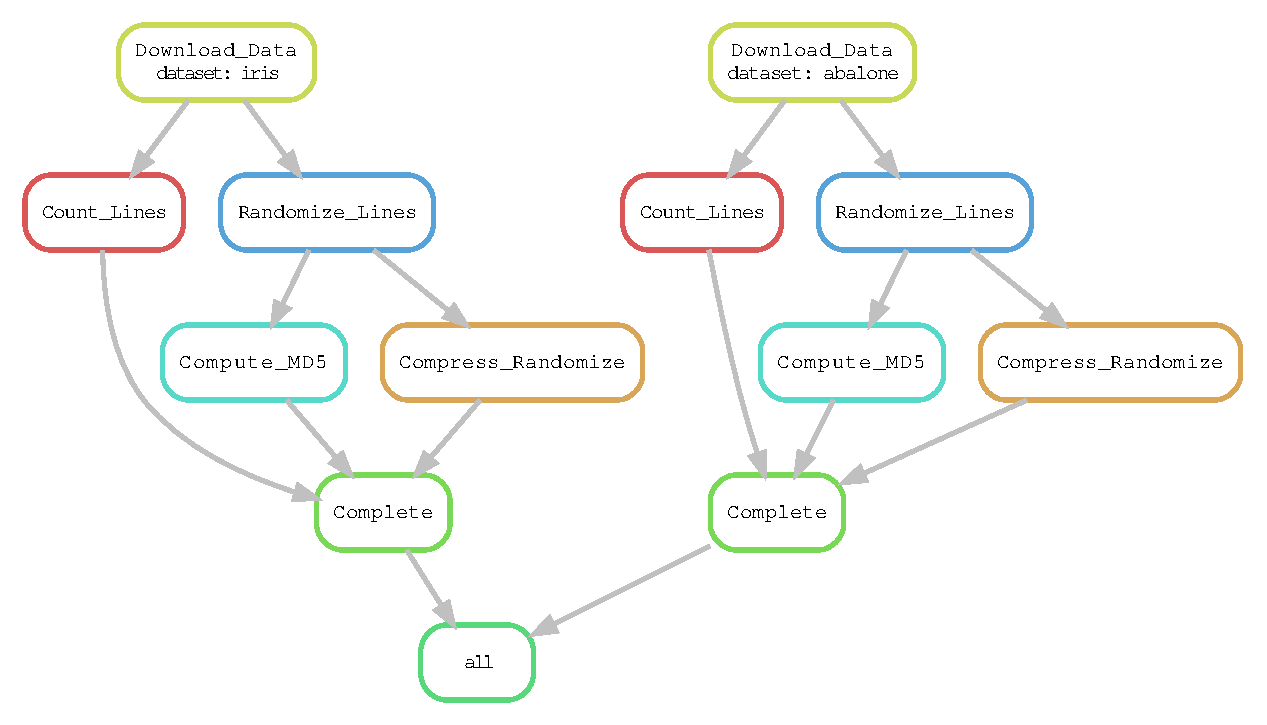
\includegraphics[width=\linewidth]{example/graph}
\end{figure}

\end{frame}


%%%%%%%%%%%%%%%%%%%%%%%%%%%%%%%%%%%%%%%%%%%%%%%%%%%%%%%
\begin{frame}

\frametitle{Other Works}

\begin{figure}
  \centering
  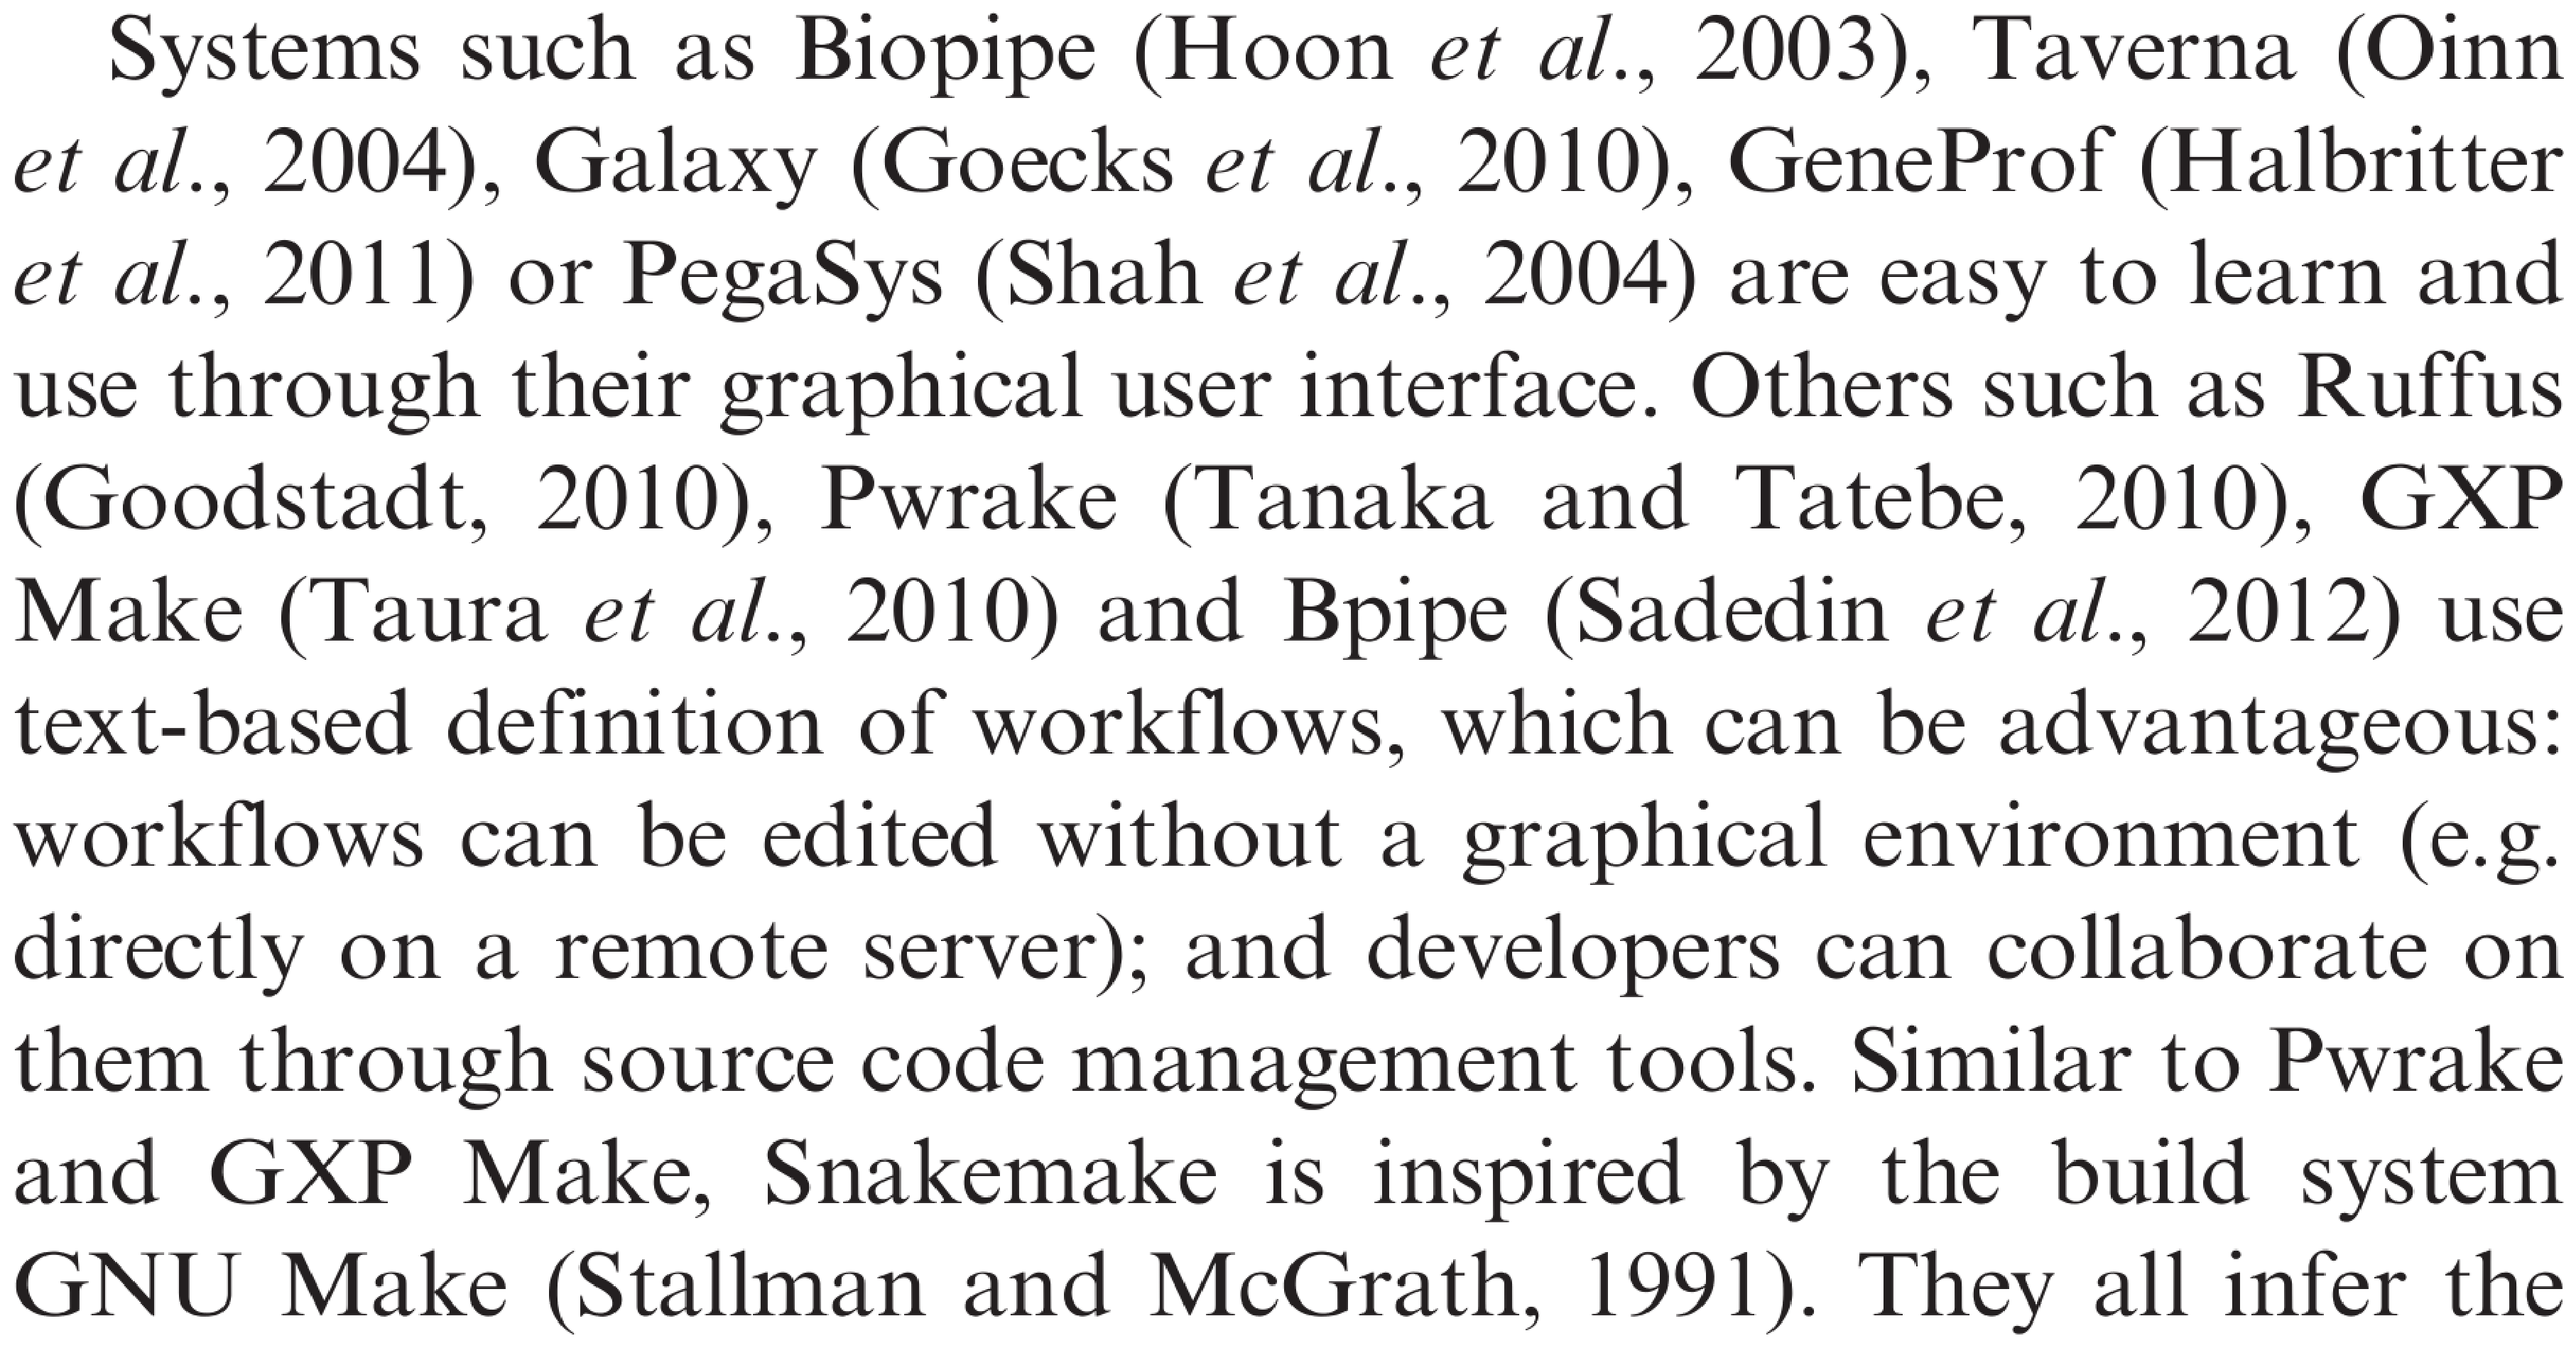
\includegraphics[width=\linewidth]{conclude/related}
\end{figure}

{\figsource{From the Snakemake paper}}

\end{frame}


%%%%%%%%%%%%%%%%%%%%%%%%%%%%%%%%%%%%%%%%%%%%%%%%%%%%%%%
\begin{frame}

\frametitle{Further Information}

More information is available from the developer:
\begin{description}
  \item[Documentation] \href{https://snakemake.readthedocs.io/en/stable/}{https://snakemake.readthedocs.io/en/stable/}
  \item[Manuscript] In Bioinformatics journal\footnote{\href{https://academic.oup.com/bioinformatics/article/28/19/2520/290322}{https://academic.oup.com/bioinformatics/article/28/19/2520/290322}}
  \item[Source] \href{https://bitbucket.org/snakemake/snakemake.git}{https://bitbucket.org/snakemake/snakemake.git}
\end{description}

\end{frame}





\end{document}


